\documentclass[conference, utf8]{IEEEtran}
\usepackage[pdftex]{graphicx}
% declare the path(s) where your graphic files are
\graphicspath{{figs/}} 
\usepackage[cmex10]{amsmath}
\interdisplaylinepenalty=2500


%\usepackage[T1,T2A]{fontenc}
%\usepackage[OT2,T1]{fontenc}
%\usepackage[utf8]{inputenc}
%\usepackage[LCY,OT1]{fontenc}
%\usepackage[OT1,LCY]{fontenc}

%OT2, LWN, LCY, X2, T2C, T2B, T2A, 
\usepackage[utf8]{inputenc}
\usepackage[OT2,OT1]{fontenc}
\usepackage[ukrainian,english]{babel}

% correct bad hyphenation here
\hyphenation{op-tical net-works semi-conduc-tor}

\begin{document}
%
% paper title
% can use linebreaks \\ within to get better formatting as desired
\title{Combined Complementary Filter For Inertial Navigation System}


% author names and affiliations
% use a multiple column layout for up to three different
% affiliations
\author{\IEEEauthorblockN{Nikolai Filiashkin}
\IEEEauthorblockA{IACS\\
National Aviation University\\
Kyiv, Ukraine}
\and
\IEEEauthorblockN{Nikolai Novik}
\IEEEauthorblockA{IACS\\
National Aviation University\\
Kyiv, Ukraine}}

% make the title area
\maketitle


\begin{abstract}
%\boldmath
This paper presents an analysis of complementary algorithm for inertial 
navigation systems. Proposed suboptimal algorithm for sensors data 
fusion of navigation system, this method employs combined complementary 
filter approach and attitude error equation of inertial navigation system. 
Simulation results are presented to demonstrate the  performance of the 
proposed approach. 
\end{abstract}
% IEEEtran.cls defaults to using nonbold math in the Abstract.
% This preserves the distinction between vectors and scalars. However,
% if the conference you are submitting to favors bold math in the abstract,
% then you can use LaTeX's standard command \boldmath at the very start
% of the abstract to achieve this. Many IEEE journals/conferences frown on
% math in the abstract anyway.

% no keywords
\begin{IEEEkeywords}
complementary filtering, inertial navigation system, data fusion
\end{IEEEkeywords}



% For peer review papers, you can put extra information on the cover
% page as needed:
% \ifCLASSOPTIONpeerreview
% \begin{center} \bfseries EDICS Category: 3-BBND \end{center}
% \fi
%
% For peerreview papers, this IEEEtran command inserts a page break and
% creates the second title. It will be ignored for other modes.
\IEEEpeerreviewmaketitle



\section{Introduction}
The traditional approach to navigation systems employ Inertial Navigation System (INS) and 
Global Navigation Satellite System(GNSS), different data fusion algorithms are used.

%The majority of navigation data fusion algorithms are based on Kalman filters, particularly 
Extended Kalman filter. The EKF linearizes both the process  and the observation functions 
%with a first-order Taylor  approximation. In practice, this approximation is the source of 
errors of the EKF [5], since the approximated none-linear problem is actually solved 
optimally by the corresponding linear Kalman filter. Besides it is difficult to know exact 
values for covariance matrix of process noise. Together, these factors contribute to filter 
divergence. 

Leading researchers solve this problem in most cases using own unique approaches. In 
particular in order to overcome divergence large amount Kalman filter modification 
was developed, for instance: Yasvinsky algorithms, different robust [3] and adaptive 
extensions [4].  

At the present time besides optimal state vector estimation (Kalmna filter), there are 
other methods of data fusion, which is well proven in practice, in particular 
complementary filters. The feasibility of this method is due to the fact that 
measurement of navigation data based on different physical principles, and 
measurement errors remain in different frequency ranges.

Complementary filter approach allows estimating only measured components of 
navigation system, in case of Kalman filter there is capability to estimate all 
components of state vector, in particular the angular orientation and sensor’s 
instrumental errors (gyro and accelerometer biases).

\section{Complementary filter}
This paper proposes the combined complementary filter: measured components of state 
vector estimated with complementary filter approach and indirectly measured attitude 
extrapolate by means of INS error equation.

As data fusion of redundant navigation information, complementary filter is proposed, 
which is well known from Doppler inertial navigation systems (Fig. 1), rather than 
reduced Kalman filter.

\begin{figure}[!t]
\centering
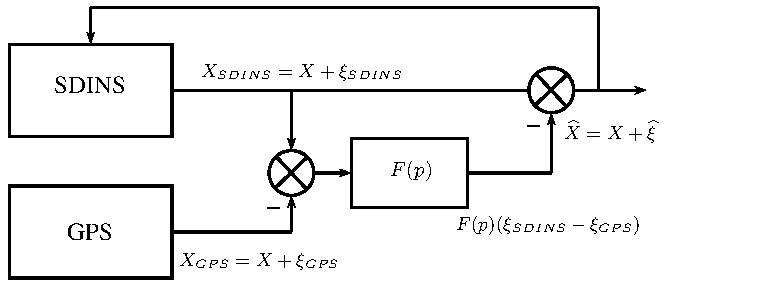
\includegraphics[width=3.5in]{f1.pdf}
\caption{Complementary filter}
\label{fig:compl}
\end{figure}

Instead of the classical aperiodic filter $F(p)$ in compensation schemes, authors 
propose to use a third order filter with variable structure.

\begin{equation}
\displaystyle F(p) = \left\{ 
    \begin{array}{ll}
       \displaystyle \frac{1}{T_{1} p+1} x & \mbox{if $t_{up} \le T_{1}$};\\
       \displaystyle \frac{T_{2} p+1}{(T_{2} p+1)(T_{2} p+1)(T_{2} p+1)} & \mbox{if $T_{1} <t_{up} \le T_{2}$};\\
       \displaystyle \frac{T_{3} p+1}{(T_{3} p+1)(T_{3} p+1)(T_{3} p+1)}& \mbox{if $T_{2} < t_{up}$}.
    \end{array} 
\right.
\label{eq:comp_f}
\end{equation}

here $t_{up}$ - uptime of compensation complementary filter. 

Studies have shown \cite{bib:rogozhyn}, such data fusion algorithm gives results not worse than the 
Kalman filtering, without affecting the stability of estimation algorithms.

\begin{figure}[!t]
  \centering
  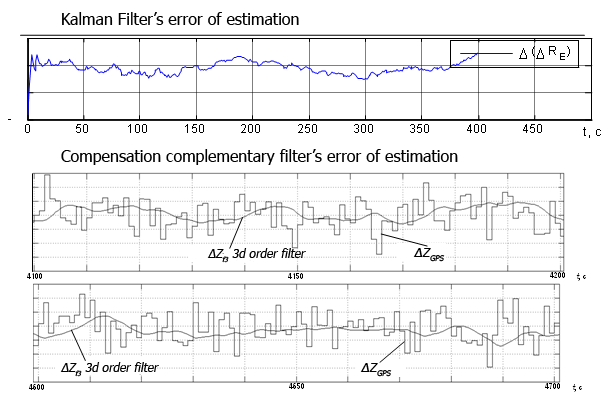
\includegraphics[width=3.1in]{f22}
  \caption{Kalman and complementary filter performance}
  \label{fig:sim_kalman}
\end{figure}

However, this algorithm does not estimate observable state vector components, in particular angular orientation.

State vector of complex inertial satellite navigation system $\bf{x_{ISNS,k}} $ 
based on error equation of inertial and stattelite systems 
${\bf x}_{ISNS;k} =
\left|\begin{array}{c} {{\bf x}_{INS,k} } \\ {{\bf x}_{GNSS,k} } \end{array}\right|$, 
by using the optimal Kalman filter, the generalized state space  equation of a complex system errors can be written as:

\begin{equation}
{\bf x}_{ISNS;k} =\Phi_{ISNS,k} {\bf x}_{ISNS;k-1} +\xi _{ISNS} 
\label{eq:state_prop}
\end{equation}
where  $\Phi_{ISNS;k} =\left|\begin{array}{cc} {\Phi_{INS,k} } & {0} \\ {0} & {\Phi_{GNSS,k} } \end{array}\right|\, -$ known 
state propagation matrix, which is formed on the basis of the$\Phi_{ISNS} $, $\Phi_{{\rm GNSS}} $ matrices, models 
of correlated components of GNSS and INS; 
$\xi _{ISNS;k} =\left|\begin{array}{c} {\xi _{INS,k} } \\ {\xi _{{\rm SNS,\; }k} } \end{array}\right|\,$  -- vector 
of zero mean white Gaussian noise with covariance matrix $Q_{ISNS;k} \, $ (process noise matrix), of two corresponding navigation systems. 

Equation for estimation of $\hat{{\bf x}}_{ISNS;k} $, with certain assumptions, derived 
from the general equations of optimal filtering and have the form:



\begin{equation} 
\label{GrindEQ__1_} 
\begin{array}{l} {\hat{{\bf x}}_{ISNS;k} =\tilde{{\bf x}}_{ISNS;k|k-1} +K_{k} (z_{GNSS,k} -\stackrel{\frown}{z}_{ISNS;k} );} \\ 
{\stackrel{\frown}{z}_{ISNS,k} =G(z_{INS,k} -_{INS,k} \tilde{{\bf x}}_{INS,k|k-1} )+_{{\rm SNS,\; }k} \tilde{{\bf x}}_{{\rm SNS,\; }k|k-1} ;} 
\end{array} \end{equation} 

\begin{equation} \label{GrindEQ__2_} \tilde{{\bf x}}_{ISNS;k|k-1} =\Phi_{ISNS;k} 
\hat{{\bf x}}_{ISNS;k-1} ;\, \tilde{{\bf x}}_{INS,k|k-1} =\Phi_{INS,k} \hat{{\bf x}}_{INS,k-1} ;\, \tilde{{\bf x}}_{{\rm SNS,\; }k|k-1} 
=\Phi_{{\rm SNS,\; }k} \hat{{\bf x}}_{{\rm SNS,\; }k-1} ; 
\end{equation} 

\[\begin{array}{l} {K_{k} =P_{k|k-1} H_{k}^{{\rm T}} (H_{k} P_{k|k-1} H_{k}^{{\rm T}} +N_{k} )^{-1} ;} \\ 
{P_{k|k-1} =\Phi_{ISNS;k} P_{k-1} \Phi_{ISNS;k}^{{\rm B}} +Q_{ISNS;k} ;} \end{array}\] 

\[\begin{array}{l} {P_{k} =P_{k|k-1} -K_{{\rm D,}\, \, \, k} H_{k} P_{k|k-1} ;} \\ 
{H_{k} =\frac{\partial }{\partial V_{ISNS;k} } \left[G(Z_{INS,k} -_{INS,k} {\bf x}_{INS,k} )+_{{\rm S}NS,\, k} 
{\bf x}_{{\rm S}NS,\, k} \right]_{{\bf x}_{{\rm I}SNS,\, k} =\tilde{{\bf x}}_{{\rm I}SNS,\, k|k-1} } ,} \end{array}\] 

%where $z_{{\rm GNSS}} $, $z_{{\rm INS}} $ $-$ observation vectors of GNSS and INS; \textbf{G }$-$ known matrix of vector function \textbf{G}(\textbf{$\hat{{\bf x}}_{ISNS;k} $}),  that connects the radio navigation signal parameters with the estimated state vector\textbf{$\hat{{\bf x}}_{ISNS;k} $}; $M_{{\rm GNSS}} $, $\, M_{{\rm INS}} $$-$ known matrices error of observation process from GNSS and INS; $\stackrel{\frown}{z}_{ISNS} $$-$ estimation of observation vector; $\tilde{{\bf x}}_{ISNS} $, $\tilde{{\bf x}}_{{\rm INS}} $, $\tilde{{\bf x}}_{{\rm SNS}} $$-$ errors of estimation of complex system, INS and GNSS errors; $\tilde{{\bf x}}_{ISNS;k|k-1} $ и $P_{k|k-1} $ $-$ corresponding errors of INS, GNSS and covariance matrix for moment \textbf{Р} \textit{k},\textit{ }calculated based on  measurements in previous time stamps\textit{ k }$-$1, \textit{k }$-$2; \textbf{Н} $-$ measurement matrix; \textbf{N} $-$ measurement noise covariance matrix.
where $z_{GNSS}$, $z_{INS}$ -- observatin vector of GNSS and INS; ${bf G}$ -- known matrix of vector function ${bf G}(\hat{{\bf x}}_{ISNS;k} $
Simulations of proposed filtering approach were done with simplified variant of inertial navigation system with following equation of motion:


\begin{equation}
\begin{array}{l}
  \displaystyle \dot{\varphi }=\frac{V_{N} }{R_{E} +h} ; \dot{h}=V_{U} ; \dot{\vartheta }=\omega -\frac{V_{N} }{R_{E} +h} ;\\
  \displaystyle \dot{V}_{N} =a_{N} -\frac{V_{N} }{R_{E} +h} V; \dot{V}_{U} =a_{U} +\frac{V_{N} }{R_{E} +h} V_{N} -g;\\
  \displaystyle a_{N} =a_{y} \cos \vartheta -a_{z} \sin \vartheta ; a_{U} =a_{y} \sin \vartheta +a_{z} \cos \vartheta ;\\
  \end{array} 
  \label{eq:ins}
\end{equation}
$\varphi$,$h$- latitude and height; 
$V_{N}$, $V_{U}$- North and Up velocity; 
$a_{N}$, $a_{U}$ - North and Up acceleration; 
$a_{y}$, $a_{z}$ - acceleration in body frame (accelerometers output); 
$\vartheta$ - pitch angle;$\omega $- angular velocity in body frame (gyro output); 
$R_{E}$- Earth radius;

For simulation purposes next parameters of inertial sensors was used:
\begin{table}[!t]\footnotesize
\centering
\renewcommand{\arraystretch}{1.3}
  \caption{Simulation Parameters}
    \begin{tabular}{|l|p{50mm}|} \hline 
      Parameter & Value \\ \hline  \hline 
      Gyro bias & $100^{\circ } /hr$ \\ \hline 
      Angular random walk & $1.2^{\circ } /\sqrt{hr} $ \\ \hline 
      Accelerometer bias & $10^{-2} g$ \\ \hline 
      Velocity random walk & $0.18m/s/\sqrt{hr} $ \\ \hline 
      GNSS position precision & $7m(1\sigma )$ \\ \hline 
      GNSS velocity precision & $0.05m/s(1\sigma )$ \\ \hline 
    \end{tabular}
  \label{tab:sim}
 \end{table}


Performance of complementary filter presented on fig.\ref{fig:coomp_v}, \ref{fig:coomp_pos}, \ref{theta_err}, and \ref{theta_err_of_err}. In particular fig. \ref{} shows the extrapolation 
of the INS angular orientation errors. 

\begin{figure}[!t]
  \centering
  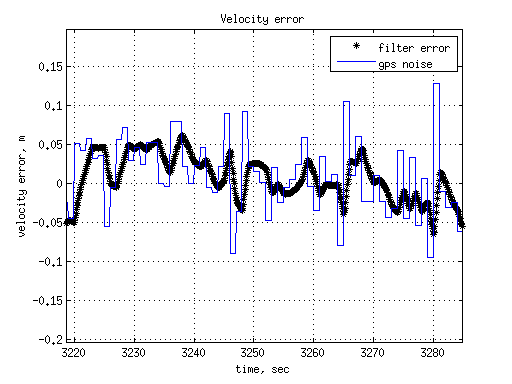
\includegraphics[width=3.1in]{vn_err_of_err}
  \caption{Figure 3.  Estimation error of velocity}
  \label{fig:coomp_v}
\end{figure}

\begin{figure}[!t]
  \centering
  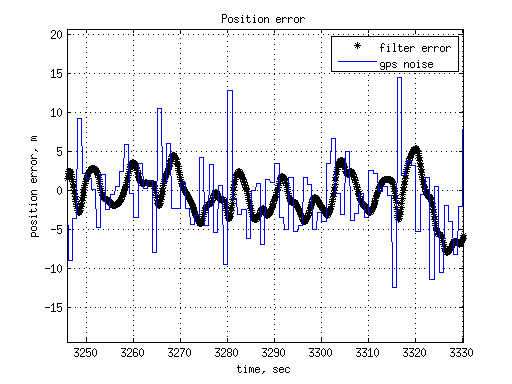
\includegraphics[width=3.1in]{phi_err_of_err}
  \caption{Figure 3.  Estimation error of positon}
  \label{fig:comp_pos}
\end{figure}

\section{ Attitude error extrapolator}

In studies of the combined complementary filter was made the following assumption: since 
from the output of complementary filter we can observe the errors evolution of inertial 
navigation system, it becomes possible to use this information to construct the attitude 
error extrapolator. Attitude errors can be described with following equation:

\begin{equation}
 \delta \dot{\vartheta }=-\frac{1}{R_{E} +h} \delta V_{N} +\frac{V_{N} }{(R_{E} +h)^{2} } \delta h+\varepsilon
 \label{eq:ins_att}
\end{equation}
$\delta h$- INS height error; 
$\delta V_{N} $- INS North velocity error; 
$\delta \vartheta $- attitude error; 
$\varepsilon $- gyro bias.

This approach makes possible to predict the INS attitude error, 
like Kalman filter does on predict stage. In case of precise initial conditions, 
it is possible to get quite accurate predictions for the pitch error on a long 
time period, even for very noisy sensors. In our case, the angular random 
walk was chosen$1.2{}^\circ /\sqrt{hr} $, for example inertial measurement 
unit Navchip (\$ 1,000) from InterSense includes micromechanical gyroscopes 
with an angular random walk$0.18{}^\circ /\sqrt{hr} $, and the device has a 
one order of magnitude lower the noise density. 

\begin{figure}[!t]
  \centering
  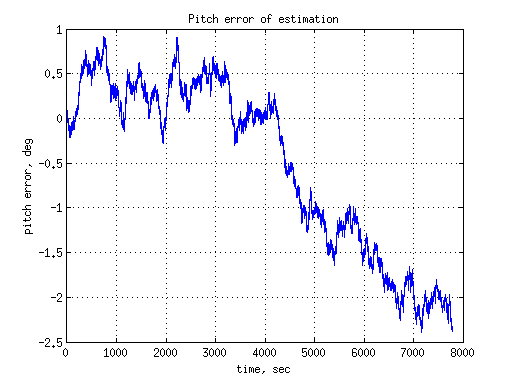
\includegraphics[width=3.1in]{theta_err_of_err}
  \caption{Attitude estimation error}
  \label{fig:theta_err_err}
\end{figure}

\begin{figure}[!t]
  \centering
  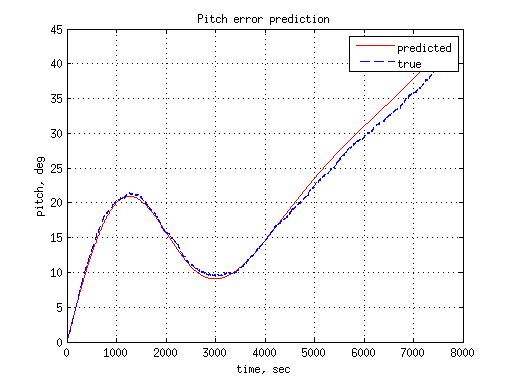
\includegraphics[width=3.1in]{theta_err}
  \caption{Prediction of  INS attitude error}
  \label{fig:theta_err}
\end{figure}

This method has several drawbacks: large sensitivity to initial conditions 
of attitude INS errors. If gyro bias set with an accuracy of 10\%, the results 
of the extrapolation of attitude error significantly deteriorate (fig. 5). 
Since no stage correction, extrapolated attitude INS error diverges with the 
time. Approach can be used quite successful in case if UAVs operation time 
or attitude correction time (for instance steady flight without acceleration) 
less then diverge time of filter.
\begin{figure}[!t]
  \centering
  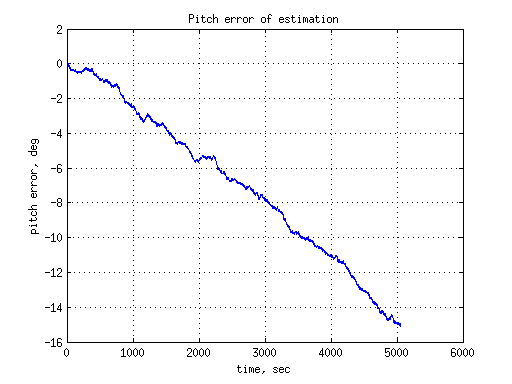
\includegraphics[width=3.1in]{theta_err_of_err_2}
  \caption{Attitude estimation error in case of 10\% error in initial condition for gyro bias}
  \label{fig:theta_err_err2}
\end{figure}

\begin{figure}[!t]
  \centering
  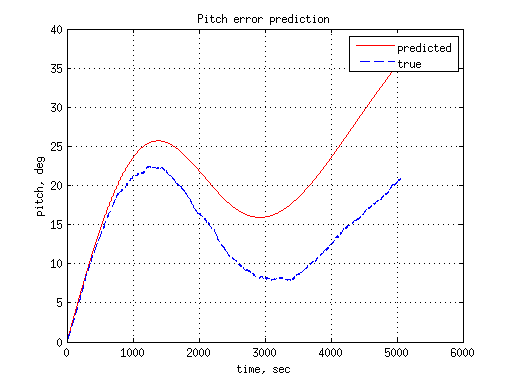
\includegraphics[width=3.1in]{theta_err_2}
  \caption{Prediction of  INS attitude error in case of 10\% error in initial condition for gyro bias}
  \label{fig:theta_err2}
\end{figure}

\section{Conclusions}
The proposed approach to state estimation and data fusion for inertial and 
satellite navigation systems is faster operating and robust to non-stationary
random processes, which are for instance sensor's scale factors or biases and 
in other hand it can be quite easy implemented in the onboard digital computer.

\begin{thebibliography}{1}

\bibitem{bib:zakharin}  \foreignlanguage{ukrainian}
{Ф.М. Захарін, В.М. Синєглазов, М.К. Філяшкін. \emph{Алгоритмічне забезпечення інерціально- супутникових систем навігаціі} - K. \:Вид-во НАУ, 2011. – 320 с.}
\bibitem{bib:rogozhyn} \foreignlanguage{ukrainian}{В.А. Рогожин, В.М. Синеглазов Н.К. Филяшкин 
\emph{Пілотажно-навігаційні комплекси повітряних суден}: К.: НАУ, 2007. – 306 с.}
\bibitem{bib:wan}E. A. Wan and R. Van Der Merwe, 
\emph{The unscented Kalman filter for nonlinear estimation}, in Adaptive Systems for Signal Processing, Communications, and Control Symposium 2000. AS-SPCC. The IEEE 2000, 2000, pp. 153–158.
\bibitem{bib:mohamed}A. H. Mohamed and K. P. Schwarz, 
\emph{Adaptive Kalman filtering for INS/GPS}, Journal of Geodesy, vol. 73, no. 4, pp. 193–203, 1999.
\bibitem{bib:toledo}R. Toledo-Moreo, D. Gruyer, and A. Lambert, 
\emph{A theoretical analysis of the Extended Kalman Filter for data fusion in vehicular positioning,} in ITS Telecommunications (ITST), 2011 11th International Conference on, 2011, pp. 305–310.


\end{thebibliography}




% that's all folks
\end{document}


